\subsection{Background Subtraction \& Foreground Detection}
\label{sec:bg_fg}
Both background and foreground are modeled using Gaussian Mixture Models (GMM), as proposed by Stauffer and Grimson \cite{stauffer1999adaptive}, a reliable technique that offers robustness against lighting changes, repetitive motions and long-term changes in the scene. It is based on the temporal observation of the pixels, and several Gaussians are used to represent either foreground or background. Gaussians are considered as background if they have high weight and low variance, and as foreground if they have low weight and high variance, and a pixel is assigned as background or foreground depending on its nearest Gaussian. \\

\noindent Once a foreground segmentation has been obtained, morphological operators are applied to improve the binary mask. First, closing and opening operators are applied to get better defined blobs. Then, a filling holes algorithm is used to avoid holes in the blobs. And last, an area filtering is used to remove the possible noise. Fig. \ref{fig:fg} shows an example of foreground detection for a frame of the highway sequence. 

\begin{figure}[h]
\centering
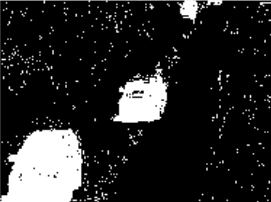
\includegraphics[width=85pt, height=75pt]{figures/fg_mask.png} 
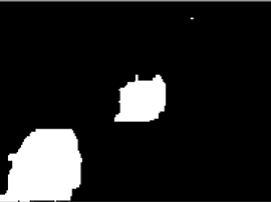
\includegraphics[width=85pt, height=75pt]{figures/fg_mask_mo.png} 
\caption{Foreground segmentation. On the left, the mask obtained with S\&G. On the right, the same mask after applying morphological operators.}
\label{fig:fg}
\end{figure}

